%
%Не забыть:
%--------------------------------------
%Вставить колонтитулы, поменять название на титульнике



%--------------------------------------

\documentclass[a4paper, 12pt]{article} 

%--------------------------------------
%Russian-specific packages
%--------------------------------------
%\usepackage[warn]{mathtext}
\usepackage[T2A]{fontenc}
\usepackage[utf8]{inputenc}
\usepackage[english,russian]{babel}
\usepackage[intlimits]{amsmath}
\usepackage{esint}
%--------------------------------------
%Hyphenation rules
%--------------------------------------
\usepackage{hyphenat}
\hyphenation{ма-те-ма-ти-ка вос-ста-нав-ли-вать}
%--------------------------------------
%Packages
%--------------------------------------
\usepackage{amsmath}
\usepackage{amssymb}
\usepackage{amsfonts}
\usepackage{amsthm}
\usepackage{latexsym}
\usepackage{mathtools}
\usepackage{etoolbox}%Булевые операторы
\usepackage{extsizes}%Выставление произвольного шрифта в \documentclass
\usepackage{geometry}%Разметка листа
\usepackage{indentfirst}
\usepackage{wrapfig}%Создание обтекаемых текстом объектов
\usepackage{fancyhdr}%Создание колонтитулов
\usepackage{setspace}%Настройка интерлиньяжа
\usepackage{lastpage}%Вывод номера последней страницы в документе, \lastpage
\usepackage{soul}%Изменение параметров начертания
\usepackage{hyperref}%Две строчки с настройкой гиперссылок внутри получаеммого
\usepackage[usenames,dvipsnames,svgnames,table,rgb]{xcolor}% pdf-документа
\usepackage{multicol}%Позволяет писать текст в несколько колонок
\usepackage{cite}%Работа с библиографией
\usepackage{subfigure}% Человеческая вставка нескольких картинок
\usepackage{tikz}%Рисование рисунков
\usepackage{float}% Возможность ставить H в положениях картинки
% Для картинок Моти
\usepackage{misccorr}
\usepackage{lscape}
\usepackage{cmap}



\usepackage{graphicx,xcolor}
\graphicspath{{Pictures/}}
\DeclareGraphicsExtensions{.pdf,.png,.jpg}

%----------------------------------------
%Список окружений
%----------------------------------------
\newenvironment {theor}[2]
{\smallskip \par \textbf{#1.} \textit{#2}  \par $\blacktriangleleft$}
{\flushright{$\blacktriangleright$} \medskip \par} %лемма/теорема с доказательством
\newenvironment {proofn}
{\par $\blacktriangleleft$}
{$\blacktriangleright$ \par} %доказательство
%----------------------------------------
%Список команд
%----------------------------------------
\newcommand{\grad}
{\mathop{\mathrm{grad}}\nolimits\,} %градиент

\newcommand{\diver}
{\mathop{\mathrm{div}}\nolimits\,} %дивергенция

\newcommand{\rot}
{\ensuremath{\mathrm{rot}}\,}

\newcommand{\Def}[1]
{\underline{\textbf{#1}}} %определение

\newcommand{\RN}[1]
{\MakeUppercase{\romannumeral #1}} %римские цифры

\newcommand {\theornp}[2]
{\textbf{#1.} \textit{ #2} \par} %Написание леммы/теоремы без доказательства

\newcommand{\qrq}
{\ensuremath{\quad \Rightarrow \quad}} %Человеческий знак следствия

\newcommand{\qlrq}
{\ensuremath{\quad \Leftrightarrow \quad}} %Человеческий знак равносильности

\renewcommand{\phi}{\varphi} %Нормальный знак фи

\newcommand{\me}
{\ensuremath{\mathbb{E}}}

\newcommand{\md}
{\ensuremath{\mathbb{D}}}



%\renewcommand{\vec}{\overline}




%----------------------------------------
%Разметка листа
%----------------------------------------
\geometry{top = 3cm}
\geometry{bottom = 2cm}
\geometry{left = 1.5cm}
\geometry{right = 1.5cm}
%----------------------------------------
%Колонтитулы
%----------------------------------------
\pagestyle{fancy}%Создание колонтитулов
\fancyhead{}
%\fancyfoot{}
\fancyhead[R]{\textsc{Подготовка к экзамену}}%Вставить колонтитул сюда
%----------------------------------------
%Интерлиньяж (расстояния между строчками)
%----------------------------------------
%\onehalfspacing -- интерлиньяж 1.5
%\doublespacing -- интерлиньяж 2
%----------------------------------------
%Настройка гиперссылок
%----------------------------------------
\hypersetup{				% Гиперссылки
	unicode=true,           % русские буквы в раздела PDF
	pdftitle={Заголовок},   % Заголовок
	pdfauthor={Автор},      % Автор
	pdfsubject={Тема},      % Тема
	pdfcreator={Создатель}, % Создатель
	pdfproducer={Производитель}, % Производитель
	pdfkeywords={keyword1} {key2} {key3}, % Ключевые слова
	colorlinks=true,       	% false: ссылки в рамках; true: цветные ссылки
	linkcolor=blue,          % внутренние ссылки
	citecolor=blue,        % на библиографию
	filecolor=magenta,      % на файлы
	urlcolor=cyan           % на URL
}
%----------------------------------------
%Работа с библиографией (как бич)
%----------------------------------------
\renewcommand{\refname}{Список литературы}%Изменение названия списка литературы для article
%\renewcommand{\bibname}{Список литературы}%Изменение названия списка литературы для book и report
%----------------------------------------
\begin{document}
	\begin{titlepage}
		\begin{center}
			$$$$
			$$$$
			$$$$
			$$$$
			{\Large{НАЦИОНАЛЬНЫЙ ИССЛЕДОВАТЕЛЬСКИЙ УНИВЕРСИТЕТ}}\\
			\vspace{0.1cm}
			{\Large{ВЫСШАЯ ШКОЛА ЭКОНОМИКИ}}\\
			\vspace{0.25cm}
			{\large{Факультет физики}}\\
			\vspace{5.5cm}
			{\Huge\textbf{{Подготовка к экзамену}}}\\%Общее название
			\vspace{1cm}
			\vspace{2cm}
			{Работу выполнил студент 3 курса}\\
			{Захаров Сергей Дмитриевич}
			\vfill
			
\includegraphics[width = 0.2\textwidth]{HSElogo}\\
			\vfill
			Москва\\
			2020
		\end{center}
	\end{titlepage}
	
\tableofcontents

\newpage

\section{Метод исследования поверхности: дифракция на медленных электронах}

\subsection{Описание и установка}

Метод заключается в анализе картин дифракции низкоуровневых электронов с энергией 30-200~эВ, упруго рассеянных от исследуемой поверхности.

Схема типичной экспериментальной установки представлена на рисунке \ref{fig:exp_setup}. В электронной пушке электроны, испускаемые катодом (находящимся под отрицательным потенциалом $-V$), ускоряются до энергии $eV$, а затем движутся и рассеиваются на образце в бесполевом пространстве, поскольку первая сетка дифрактометра и образец заземлены. Вторая и третья сетки, находящиеся под потенциалом чуть меньше потенциала катода ($V - \Delta V$), служат для отсечения неупруго рассеянных электронов. Четвертая сетка заземлена и экранирует другие сетки от флуоресцентного экрана, находящегося под потенциалом порядка +5 кВ. Таким образом, электроны, упруго рассеянные на поверхности образца, после прохождения тормозящих сеток ускоряются до высоких энергий, чтобы вызвать флуоресценцию экрана, на котором и наблюдается дифракционная картина. Экран может заменяться матрицей.

\begin{figure}[H]
	\centering
	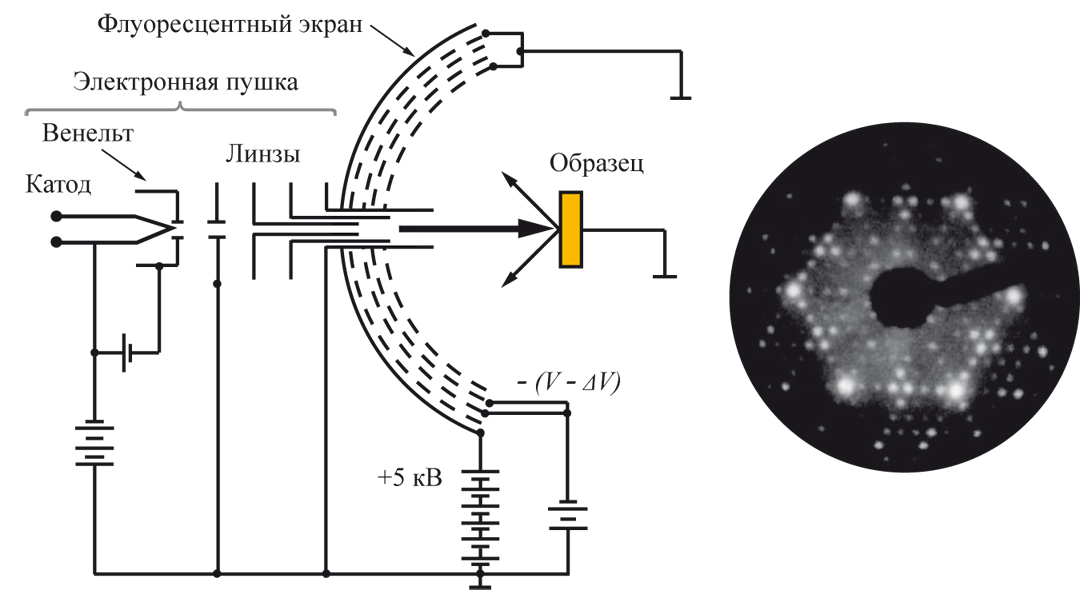
\includegraphics[width=0.8\linewidth]{Slow_electrons}
	\caption{Схема экспериментальной установки для прямого наблюдения картин ДМЭ}
	\label{fig:exp_setup}
\end{figure}

\subsection{Почему используются низкие энергии?}

\begin{enumerate}
	\item Длина волны де-Бройля для электронов с энергией 30–200 эВ составляет примерно 0.1-0.2 нм, что удовлетворяет условию дифракции на атомных структурах, а именно, длина волны равна или меньше межатомных расстояний.
	
	\item Средняя длина пробега таких низкоэнергетических электронов составляет несколько атомных слоев. Вследствие этого большинство упругих рассеяний происходит в самых верхних слоях образца (которые нас и интересуют), следовательно, они дают максимальный вклад в картину дифракции.
\end{enumerate}

\subsection{Что позволяет?}

\begin{enumerate}
	\item Качественно оценить структурное совершенство поверхности — от хорошо упорядоченной поверхности наблюдается картина ДМЭ с четкими яркими рефлексами и низким уровнем фона.
	
	\item Определить обратную решетку поверхности из геометрии дифракционной картины.
	
	\item Определить атомную структуру поверхности путем сравнения зависимостей интенсивности дифракционных рефлексов от энергии электронов, рассчитанных для структурных моделей, с зависимостями, полученными в эксперименте.
	
	% Оценить морфологию поверхности по профилю дифракционного рефлекса
\end{enumerate}

\subsection{Отличия от дифракции быстрых электронов}

Методы дифракции медленных и быстрых электронов различаются энергией используемых электронов и, соответственно, различной геометрией (в ДМЭ пучок электронов падает на исследуемую поверхность практически перпендикулярно, а в ДБЭ под скользящим углом порядка $1-5 ^\circ$). Оба метода дают сходную информацию о структуре поверхности. Преимуществом ДМЭ является более простая конструкция, а также более наглядная и удобная для интерпретации получаемая информация.
%Преимущество ДБЭ заключается в возможности проведения исследований непосредственно в ходе наращивания пленок на поверхности образца.

\section{Основы двумерной кристаллографии}

В кристаллографии принята система координат, представленная на рисунке \ref{fig:coord_axes}. В общем случае она не всегда прямоугольная. 

\begin{figure}[H]
	\centering
	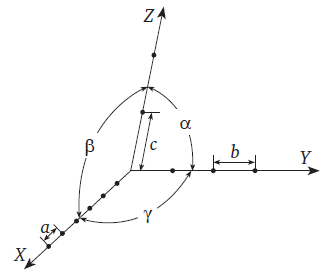
\includegraphics[width=0.5\linewidth]{Coord_axes}
	\caption{$a, b, c$ --- масштабы по осям координат; $\alpha, \beta, \gamma$ --- углы между осями координат}
	\label{fig:coord_axes}
\end{figure}

Положение любого узла представимо в виде:

\begin{equation*}
	\vec{r} = \vec{a}m + \vec{b}n + \vec{c}p
\end{equation*}

$m, n, p$ --- целые числа. При обозначении индексы узла заключаются в двойные скобки (см. рисунок \ref{fig:coord}).

% Если в одинарных, то это индексы Вейса

\begin{figure}[H]
	\centering
	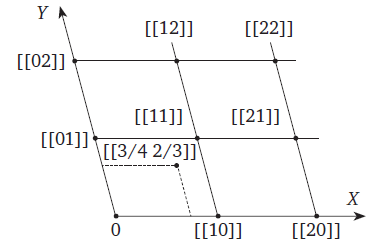
\includegraphics[width=0.5\linewidth]{Coordinates}
	\caption{Пример обозначения узлов на плоской решетке}
	\label{fig:coord}
\end{figure}

\subsection{Индексы Миллера}

Пусть есть плоскость, пересекающая оси координат на координатах $x_1, x_2, x_3$. Возьмем обратные величины и умножим на такое число, чтобы получилось минимальное целое:

\begin{equation}
	h = \frac{N}{x_1} \quad k = \frac{N}{x_2} \quad l = \frac{N}{x_3}
\end{equation}

Эти штуки называются \textbf{Индексами Миллера} и записываются в круглых скобках: $(hkl)$. Созданы из канонического уравнения плоскости.

\section{Симметрия кристаллов}

Симметрия кристаллов выделяется с помощью элементов симметрии:

\begin{enumerate}
	\item Центра симметрии
	
	\item Плоскостей симметрии
	
	\item Осей симметрии
\end{enumerate}

\subsection{Центр симметрии}

Центр симметрии (инверсии) связывает противоположные инверсионно равные (или обращено равные) части кристалла. Он совпадает с геометрическим центром кристалла. От слова Centrum он обозначается буквой С (по символике Бравэ) или $\bar{1}$ (по интернациональной символике).

При наличии центра симметрии все диаметрально противоположные грани и ребра кристалла должны быть попарно инверсионно равны и параллельны. Это на пальцах можно проверить, положив кристалл на горизонтальную плоскость стола. Если все грани и ребра кристалла попарно параллельны и инверсионно равны, центр симметрии в кристалле есть. Если центр симметрии отсутствует, то в таком кристалле сверху окажется вершина, ребро, наклонная или параллельная, но не равная нижней, грань. Наличие или отсутствие в кристалле центра симметрии следует зафиксировать в рабочей таблице.

\subsection{Плоскость симметрии}

Плоскость симметрии делит кристалл на две зеркально-равные половины. Плоскость симметрии связывает зеркально равные части кристалла. От слова Planum обозначается буквой Р (по Бравэ), от слова mirror (зеркало, отражать) обозначается буквой m (интернационально), графически обозначается сдвоенной линией (как двухсторонне зеркало).

Для определения плоскости симметрии кристалл мысленно рассекается плоскостью, проходящей через его центр. Если при этом слева и справа от плоскости симметрии все части кристалла (грани, ребра, вершины) будут повторяться как предмет и его зеркальное отображение, то такая плоскость будет являться плоскостью симметрии.
В прямоугольнике (см. рисунок \ref{fig:rect}) можно провести только две плоскости симметрии. Плоскость, делящая прямоугольник на две равные части, но не зеркально, не является плоскостью симметрии.

\begin{figure}[H]
	\centering
	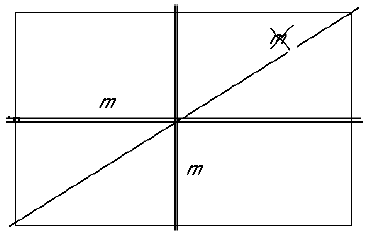
\includegraphics[width=0.5\linewidth]{Rectangle}
	\caption{Плоскости симметрии прямоугольника}
	\label{fig:rect}
\end{figure}

Куб (см. рисунок \ref{fig:cube}) имеет 9 плоскостей симметрии: три- координатных Р (слева), шесть диагональных Р (справа).

\begin{figure}[H]
	\centering
	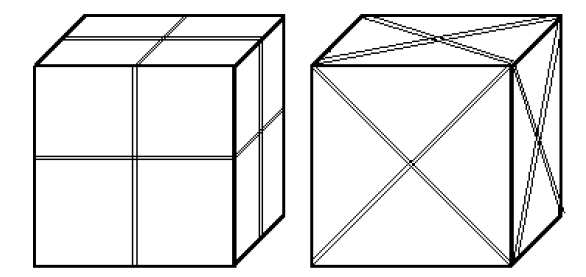
\includegraphics[width=0.5\linewidth]{Cube}
	\caption{Плоскости симметрии куба}
	\label{fig:cube}
\end{figure}

\subsection{Оси симметрии}

Ось симметрии - это линии, которые симметрично связывает конгруэнтно равные (совместимо равные) части кристалла.
Вокруг оси симметрии на равных угловых и линейных расстояниях располагаются конгруэнтно равные части кристалла, так что при полном повороте вокруг оси (на 360$^\circ$) они повторяются $n$ раз. Такие оси называют поворотными осями симметрии $n$-го порядка.

В некоторых кристаллах, помимо поворотных осей симметрии, могут быть инверсионные оси симметрии, в которых операция симметричного поворота вокруг оси совмещается с операцией симметричного отражения в центре кристалла. Порядок инверсионной оси удваивается по сравнению с порядком поворотной оси.

По Браве от слова Linie они обозначаются L$n$ (читается - ось симметрии $n$-го порядка). В кристаллах могут быть поворотные оси симметрии первого L1, второго L2, третьего L3, четвертого L4, шестого L6 порядков и инверсионные оси симметрии Li1, Li2, Li3, Li4, Li6. Кроме того, Li1 = С, Li2 = P, Li3 = L3C, Li4 = L2, Li6 = L3P.

По интернациональной символике поворотные оси симметрии обозначаются числом, указывающим их порядок, т.е. 1, 2, 3, 4 и 6, а инверсионные оси симметрии --- $\bar{1}$, $\bar{2}$, $\bar{3}$, $\bar{4}$ и $\bar{6}$.

Графически оси симметрии обозначаются многоугольником, число углов которого равно порядку оси симметрии.

В кубе: ЗL4 - (3 оси симметрии 4-го порядка) проходят через середины противоположных квадратных граней; 4L3 - (4 оси симметрии 3-го прядка) проходят через противоположные вершины; 6L2 - (6 осей симметрии 2-го прядка) проходят через середины противоположных ребер куба.

Для объяснения "на пальцах" полезно запомнить, что концы осей симметрии в кристаллах могут выходить через вершины, через центры граней и через середины ребер. Следовательно, при определении осей симметрии именно за эти элементы и нужно брать кристалл двумя пальцами и вращать его вокруг этой оси.

\textbf{Есть еще трансляционная симметрия} --- про параллельный перенос. Она запрещает L5.

\section{Геометрическая интерпретация условий дифракции по Эвальду}

Условия главных максимумов записывается в следующем виде:

\begin{equation}
	\frac{\vec{s} - \vec{s}_0}{\lambda} = \vec{H} \quad \text{или} \quad \vec{K} - \vec{K}_0 = \vec{H}
\end{equation}

Вторая версия фактически означает, что три волновых вектора ($\vec{K}_0$ --- падающий, $\vec{K}$ --- дифрагированный и $\vec{H}$ --- вектор обратной решетки, который перпендикулярен плоскостям прямой решетки с индексами ($hkl$)) связаны между собой в виде треугольника и лежат в одной плоскости, как это показано на рисунке \ref{fig:difraction}.

\begin{figure}[H]
	\centering
	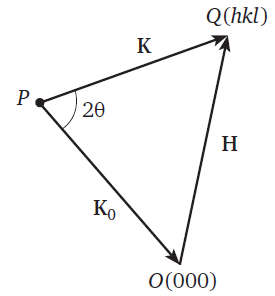
\includegraphics[width=0.5\linewidth]{Difraction}
	\caption{Векторное условие образования максимумов}
	\label{fig:difraction}
\end{figure}

\subsection{Сфера Эвальда}

Рассмотрим какую-то обратную решетку (см. рисунок \ref{fig:evald}). Из любой ее точки $P$ проведем волновой вектор падающей волны $\vec{K}_0$ в любой узел обратной решетки, который в дальнейшем будем называть нулевым узлом обратной решетки $O(000)$.

\begin{figure}[H]
	\centering
	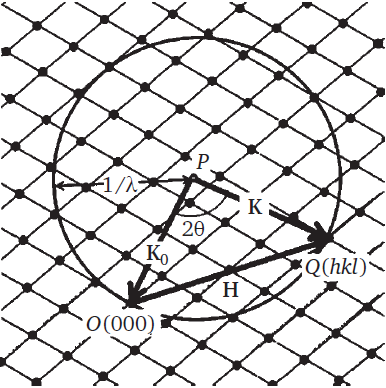
\includegraphics[width=0.5\linewidth]{Evald}
	\caption{Геометрическая интерпретация условий дифракции (сфера Эвальда)}
	\label{fig:evald}
\end{figure}

Учтем, что каждый узел обратной решетки --- система параллельных плоскостей в прямой решетке с индексами ($hkl$) и расстоянием между плоскостями $d = 1 / |H|$. Вокруг точки $P$ проведем сферическую поверхность радиусом $|K_0| = 1/\lambda$. Эта поверхность называется \textbf{сферой Эвальда}.

Будем поворачивать обратную решетку вокруг точки нулевого узла обратной решетки $O(000)$ так, чтобы на ее поверхность попадали различные узлы обратной решетки, например какой-то узел $Q(hkl)$. В таком случае при пересечении сферы Эвальда с любым узлом образуется треугольник из трех векторов $\vec{K}$, $\vec{K}_0$, $\vec{H}$. Это значит, что для системы плоскостей с индексами $(hkl)$ выполнено условие дифракции.

\subsection{Сфера ограничения}

Наряду со сферой Эвальда в структурном ана- лизе вводится понятие сферы ограничения. Эта сфера имеет радиус $R_2 = 2/\lambda$. Она строится из точки $О(000)$. Физический смысл такой конструкции состоит в том, что все узлы обратной решетки, попадающие внутрь сферы ограничения, обязательно принимают участие в формировании дифракционной картины для данной длины волны $\lambda$. Взаимное расположение сферы Эвальда и сферы ограничения представлено на рисунке \ref{fig:evald_limit}.

\begin{figure}[H]
	\centering
	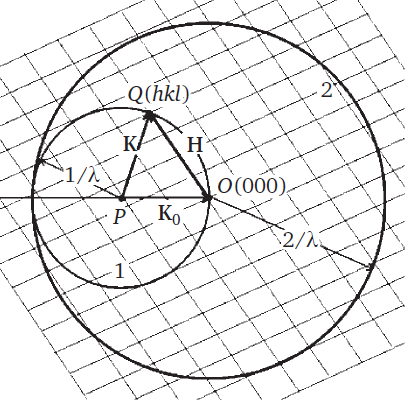
\includegraphics[width=0.5\linewidth]{Evald_limit}
	\caption{Взаимное расположение сферы Эвальда и сферы ограничений}
	\label{fig:evald_limit}
\end{figure}
 

\end{document}